\part{Contribuições para outros projetos}

	\chapter{Breve descrição sobre o projeto de fibrose cística} \index{fibrose cística}

	Durante a execução do projeto de doutorado, foi estabelecida uma parceria com uma aluna de doutorado da Faculdade de Ciências Médicas na Unicamp, Carla Cristina S. Gomez, através do Professor Francisco Benedito Pessine, do Instituto de Química da Unicamp, para a análise de amostras de muco de pacientes com fibrose cística. Nesta seção, uma pequena descrição sobre o projeto será apresentada, a contribuição do aluno será realçada, e os resultados do projeto serão mencionados.
	
	Uma alteração genética no gene que controla a produção da proteína CFTR (Cystic Fibrosis Transmembrane Conductante Regulator)\cite{Zielenski2000}, pode causar uma disfunção do transporte de íons cloreto.\cite{Quinton2008} Essa alteração genética resulta numa série de problemas corporais, e essa doença é conhecida de forma geral como fibrose cística. Há grande variação na incidência dessa doença, mas, de forma geral, pessoas Caucasianas possuem uma incidência maior.\cite{Zielenski2000}
	
	Além de afetar o transporte de cloreto, recentemente foi notado que a secreção de bicarbonato na superfície das vias aéreas é bloqueada.\cite{Quinton2001}  Isso resulta em mais íons cálcio livres e uma capacidade tamponante enfraquecida. As mucinas, componentes do muco, secretadas para lubrificar o epitélio e servir como barreira contra patógenos, são afetadas pelo excesso de Ca\textsuperscript{2+} e pelo pH baixo. Ocorre sua desidratação, tornando o muco mais espesso, comprometendo sua função de lubrificação.\cite{Quinton2008} Além disso, o pH baixo leva a uma promoção do crescimento de bactérias, acarretando na formação de biofilme e alteração da resposta imunológica.\cite{Dorschner2006}
	
	A principal causa de mortalidade da fibrose cística é a deterioração da função pulmonar através da inflamação e infecção das vias aéreas.\cite{Quinton2001} Logo, se os sintomas causados pela fibrose cística no pulmão forem eficientemente combatidos, haveria uma melhoria tanto na qualidade quanto na expectativa de vida dos pacientes. Poucos estudos testaram o efeito do bicarbonato nas vias aéreas, porém observou-se que o bicarbonato possui efeitos positivos.\cite{Stigliani2016} Os efeitos em potencial são: redução da viscosidade do muco, melhorando a lubrificação, diminuição das feridas causadas pela tosse, e remoção de detritos dos pulmões, além de aumento o pH, diminuindo a proliferação bacteriana. Logo, um estudo para verificar se essas alterações no muco pela inalação de bicarbonato afetariam positivamente os pacientes, e se a inalação em si é tolerável, é importante. Este é o primeiro estudo \emph{in vivo} dessa natureza.
	
	Uma série de 19 voluntários com fibrose cística participaram do estudo, porém 7 descontinuaram. Eles foram dosados com soluções 4,2\% e 8,4\% de NaHCO\textsubscript{3} diluído em água destilada, por inalação, e depois de duas triagens, recebiam o produto para realizar a inalação domiciliarmente. Após isso, retornavam ao centro de pesquisa para escarrar, a cada meia hora, e o muco era coletado e depois analisado. Primeiramente o pH era medido, e depois as amostras eram enviadas para serem analisadas no instituto de química. Os parâmetros das análises foram determinados pelo autor da tese, e aproximadamente metade das amostras foram analisadas pelo mesmo (cerca de 250). As amostras restantes foram analisadas pela aluna Carla Gomez. Após isso, os resultados foram tratados, e o processo de tratamento de dados será descrito nesta parte.


	\chapter{Contribuições ao projeto}
	
	Nesse projeto, foram analisados tanto curvas de fluxo, como a reologia oscilatória do muco. Utilizou-se tanto o reômetro Haake RheoStress1 quanto o Haake Mars III, ambos da Thermo Scientific, para as análises. Para o tratamento de dados, foi utilizado a linguagem Python, que permite resultados consistentes e de melhor qualidade, se comparados com o ajuste manual.
	
		\section{Determinação dos parâmetros de análise}
		
		Foram analisadas algumas amostras inicialmente para se determinar as faixas de varredura para os estudos reológicos. Primeiramente, a faixa linear de tensão foi determinada com uma varredura de 0,01 Pa a 0,75 Pa, a 1 Hz. Após isso, a varredura oscilatória de frequência foi medida, geralmente com tensões de 0,5 Pa, entre 0,1 Hz a 5 Hz. As curvas de fluxo foram medidas entre 0,01 a 1 s\menosUm.
	
		\section{Criação de um software para tratamento de curvas de fluxo} \index{resultados!curvas de fluxo}
		\label{sec:apn_tratamento_CF}
		Para o tratamento de dados de curva de fluxo, foi criado um programa que permite o usuário aplicar três modelos mais complexos, descritos na \autoref{sec:modelagem_curva_fluxo} e um modelo simplificado, o linear, para a obtenção de valores de viscosidade no repouso. Todas as amostras de muco, sem exceção, demonstraram ser pseudoplásticas, então não foram colocados mais modelos. A seguir, será mostrada somente a lógica do programa, pois o código fonte inteiro é longo demais para ser incluído aqui (aproximadamente 1000 linhas).
		
		De maior interesse para os estudos neste trabalho é a viscosidade no repouso, \(\eta_0\), e portanto esse é o foco do programa. Porém, o ajuste indiscriminado de um modelo a um dado experimental é problemático caso a qualidade do dado não seja boa, seja pela própria característica da amostra, ou pela sensibilidade do equipamento. Por exemplo, é frequente que apareçam artefatos de medida em baixos valores de \(\dot{\gamma}\), resultando ou num decréscimo ou acréscimo gradual de \(\eta\). Além disso, é possível que não seja observada a região descrita por \(\eta_{\infty}\), em altos valores de \(\dot{\gamma}\), o que atribui grande incerteza na determinação desse parâmetro. Dessa forma, é necessário que uma região das curvas seja escolhida para que o ajuste seja bem sucedido e informativo, o que representa a maior dificuldade nesse tipo de análise, devido à certa subjetividade no critério de escolha da região de ajuste. %Observando-se como os modelos variam com os parâmetros, nota-se que a queda de viscosidade do modelo de Carreau é menos abrupta que no modelo de Cross e se assemelha mais aos dados estudados, então esse modelo foi mais utilizado.
		
		Por essa razão, e outras, como velocidade de análise, foi escrito o método de ajuste. O método consiste em realizar ajustes sucessivos, entre um ponto inicial \(P_i\) até um ponto final \(P_f\), e depois comparar os resultados dos ajustes para escolher um deles. Podem ser comparados, por exemplo, os parâmetros \(R^2\), \(\chi^2\) ou \(\chi_{red}^2\). Escolhido o melhor ajuste, observando-se, por exemplo, a maior proximidade de \(R^2\) a 1 ou de \(\chi^2\) a 0, tomando cuidado para não escolher uma faixa muito estreita de pontos, os resultados são graficados, gravados num arquivo de texto e passa-se para o próximo dado experimental.
		
		A listagem \ref{lst:exemplo_curva_de_fluxo} mostra duas seções do código completo do programa, uma mostrando o ciclo de ajuste utilizando o ajuste linear e \texttt{curve\_fit} e outro que realiza um ajuste não-linear utilizando o modelo de Carreau e \emph{lmfit}.
		
		\begin{listing}[h]
			\inputminted{python}{./python/curva_de_fluxo.py}
			\caption{Seções do código mostrando o método de ajuste}  % todo: encontrar um nome melhor
			\label{lst:exemplo_curva_de_fluxo}
		\end{listing}
		
		Essas funções estão dentro de uma classe chamada \texttt{Fitter}. Para utilizar essa classe em outros códigos, é necessário inicializar uma instância da classe \texttt{Settings} e depois inicializar uma instância da classe \texttt{Fitter} utilizando as configurações da classe \texttt{Settings}. Caso não haja um arquivo \texttt{settings.dat} na pasta, um arquivo com valores padrão será criado. Após isso, é possível tanto editar o arquivo \texttt{settings.dat} quando utilizar as funções \texttt{print\_settings, edit\_settings} do objeto \texttt{Settings}. Ao criar um objeto \emph{Fitter}, por padrão os ajustes configurados já são realizados e os resultados são mostrados na tela. Caso se deseja criar um gráfico mostrando o resultado dos ajustes, pode-se chamar a função \texttt{plot\_error\_graphs()}. 
		
		A listagem \ref{lst:exemplo_fitter} mostra como o programa pode ser utilizado por outros scripts, e o resultado do ajuste se encontra na \autoref{fig:reologia_dado-exemplo}
		
		\begin{listing}[h]
			\inputminted{python}{./python/uso_fitter.py}
			\caption{Exemplo de como utilizar a ferramenta de ajuste não linear}  % todo: encontrar um nome melhor
			\label{lst:exemplo_fitter}
		\end{listing}
		
		\begin{figure}[h]
			\centering
			\includegraphics[width=\textwidth]{imagens/reologia/Dado-exemplo}
			\caption{Figura resultante do ajuste não linear de Carreau e ajuste linear gerada pela função \texttt{plot\_error\_graphs()}. As barras de erro são oriundas da propagação de erro dos parâmetros e os números em vermelho indicam os pontos iniciais e finais considerados em cada ajuste.}
			\label{fig:reologia_dado-exemplo}
		\end{figure}
		
		Note que no dado utilizado, não há muitos problemas de desvio da curva, então os ajustes foram bem comportados. Os exemplos das Figuras \ref{fig:reologia_dado-problemadescida} e \ref{fig:reologia_dado-problemasubida} mostram problemas reais na região de baixos valores de \(\dot{\gamma}\).
		
		\begin{figure}
			\centering
			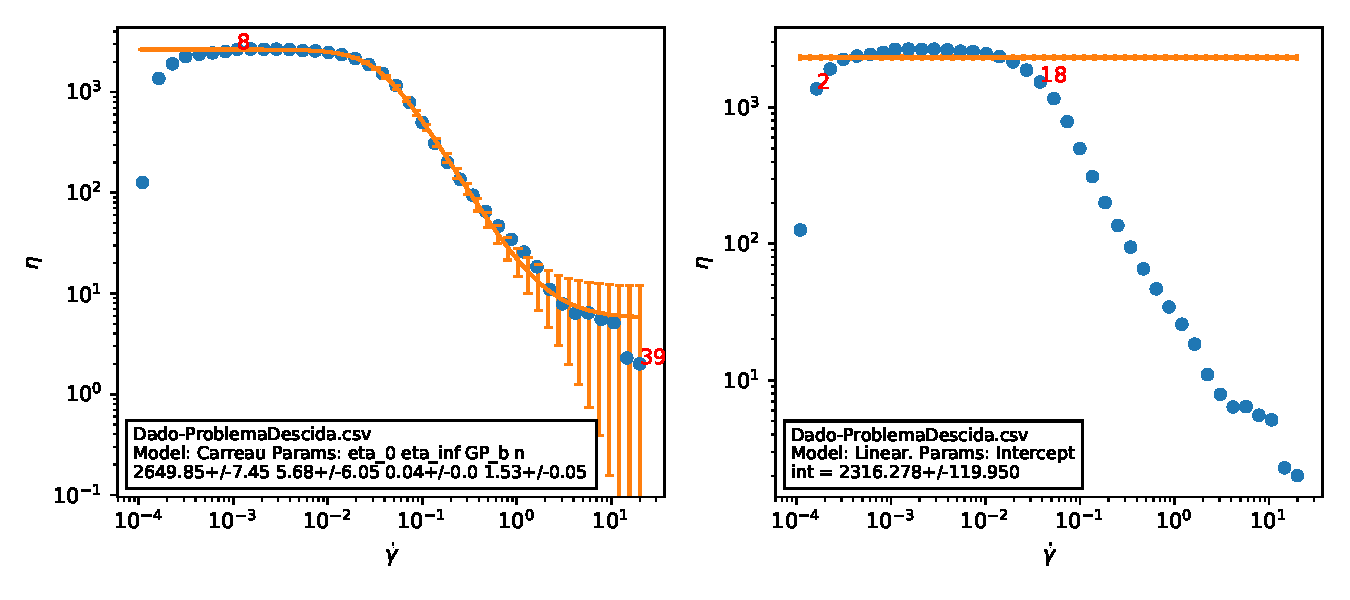
\includegraphics[width=\textwidth]{imagens/reologia/Dado-ProblemaDescida}
			\caption{Exemplo dos ajustes não-linear e linear de um dado real que possui uma queda nos valores de \(\eta\) em baixas \(\dot{\gamma}\)}
			\label{fig:reologia_dado-problemadescida}
		\end{figure}
		
		\begin{figure}
			\centering
			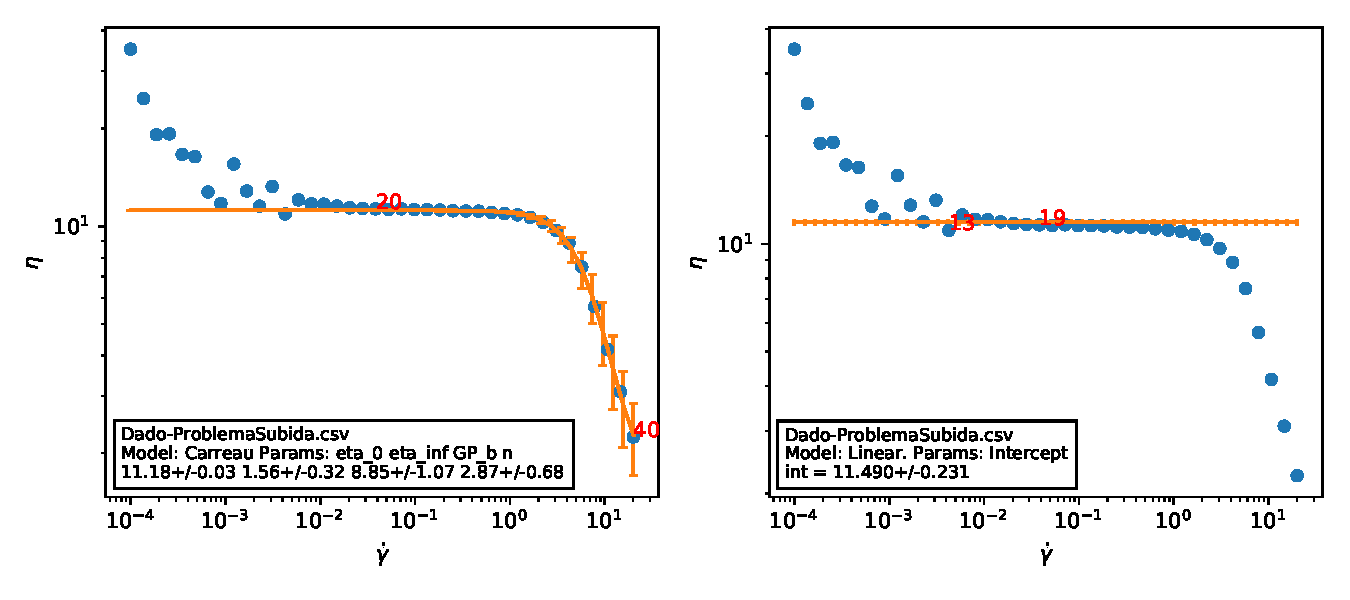
\includegraphics[width=\textwidth]{imagens/reologia/Dado-ProblemaSubida}
			\caption{Exemplo dos ajustes não-linear e linear de um dado real que possui um aumento nos valores de \(\eta\) em baixas \(\dot{\gamma}\)}
			\label{fig:reologia_dado-problemasubida}
		\end{figure}
		
		O tempo de execução e de plotagem para cada experimento está na faixa de um segundo, o que é muito mais rápido do que realizar o ajuste manualmente em uma ferramenta como o Origin ou Excel, então é algo ideal para o tratamento de um grande volume de dados.
		
	%	\FloatBarrier

		\section{Método de ajuste para reologia oscilatória de muco}
		
		As amostras de muco não seguiram modelos de reologia parecidos aos apresentados neste trabalho, como o modelo de Maxwell. Portanto, foi necessário desenvolver uma nova abordagem para analisar as amostras. Plotando-se todos os dados obtidos, observou-se que G' estava sempre acima de G'' e, na escala logarítmica, as duas curvas eram praticamente paralelas e ligeiramente inclinadas positivamente. Em alguns casos, a inclinação aumentava em frequências maiores e, frequentemente, havia uma oscilação de G' e G'' sem significado físico nessa região. A taxa de aumento era consistente com uma exponencial. Visto isso, foi desenvolvido um script que realiza o seguinte:
		
		\begin{enumerate}
			\item Obter a região de frequência confiável de G' e de G'' para o modelo linear e exponencial. Isso é feito realizando-se ajustes gradativos, do primeiro ponto até um ponto \emph{n}, armazenando os ajustes e depois escolhendo o ajuste com maior número de pontos onde \(R^2 > 0{,}9\). Caso não exista ajuste seguindo esse critério, escolhe-se um novo critério com \(R^2 > 0,85\). Caso não exista ajuste que obedeça isso mesmo assim, é escolhido o ajuste com o maior número de pontos. 
			\item Os parâmetros dos ajustes que passaram pelo filtro de \(R^2\) são gravados em um arquivo \texttt{csv}. Além disso, são gravados a média dos valores de G' e G'' da região linear, o desvio dessa média, o valor de \(R^2\), os índices dos pontos utilizados para o ajuste e o valor de G' e G'' em 0,6813Hz. Esses parâmetros foram escolhidos com base em alguns artigos da literatura. % todo: ref?
		\end{enumerate}
		
		Cerca de 500 dados experimentais únicos são tratados e plotados em cerca de 3 minutos, mostrando novamente o ganho enorme de eficiência com métodos computacionais. O código fonte da parte de tratamento de dados está nas listagens \ref{lst:extracao_muco1} -- \ref{lst:extracao_muco6}.
		
		\begin{listing}[h]
			\inputminted{python}{./python/extracao_muco1.py}
			\caption{Código fonte para a extração de informações de reologia oscilatória de muco (1/6)} 
			\label{lst:extracao_muco1}
		\end{listing}
		
		\begin{listing}[h]
			\inputminted{python}{./python/extracao_muco2.py}
			\caption{Código fonte para a extração de informações de reologia oscilatória de muco (2/6)} 
			\label{lst:extracao_muco2}
		\end{listing}
		
		\begin{listing}[h]
			\inputminted{python}{./python/extracao_muco3.py}
			\caption{Código fonte para a extração de informações de reologia oscilatória de muco (3/6)} 
			\label{lst:extracao_muco3}
		\end{listing}
		
		\begin{listing}[h]
			\inputminted{python}{./python/extracao_muco4.py}
			\caption{Código fonte para a extração de informações de reologia oscilatória de muco (4/6)} 
			\label{lst:extracao_muco4}
		\end{listing}
		
		\begin{listing}[h]
			\inputminted{python}{./python/extracao_muco5.py}
			\caption{Código fonte para a extração de informações de reologia oscilatória de muco (5/6)}
			\label{lst:extracao_muco5}
		\end{listing}
		
		\begin{listing}[h]
			\inputminted{python}{./python/extracao_muco6.py}
			\caption{Código fonte para a extração de informações de reologia oscilatória de muco (6/6)} 
			\label{lst:extracao_muco6}
		\end{listing}
		
		\FloatBarrier
		
		\chapter{Resultado da colaboração} \index{resultados!colaboração}
		
		A muco é bastante heterogêneo, dependendo da concentração de diversas espécies, como eletrólitos e pH, e também possui regiões com maior concentração de saliva. A parte mais líquida era removida durante a análise no reômetro pelo simples ato de colocar a geometria na superfície da amostra. A secagem da amostra poderia descaracterizá-la, invalidando os resultados. Além disso, cada coleta de muco fornece o muco de regiões diferentes do pulmão, levando a uma variabilidade natural alta.
		
		Essa alta variabilidade tornou a análise estatística dos dados muito difícil, então consultores externos foram utilizados. Notou-se que não houve variação significativa da viscosidade, utilizando qualquer um dos três modelos complexos e o ajuste linear.  Porém, houve correlação entre os valores de G', G'' e G\(^*\) à medida que o tratamento ocorria. De todas os fatores estudados, o pH mais fortemente se correlacionou ao tratamento, o que acabou resultando numa diminuição nos casos de infecção entre os pacientes.
		
		Porém, a parte mais relevante é a qualidade de vida dos pacientes. Todos demonstraram melhora, inclusive alguns pacientes saíram da fila de transplante por terem melhorado significativamente. No total, o estudo foi muito bem sucedido, e estudos de continuação serão realizados utilizando, também, reologia, continuando a colaboração entre os dois laboratórios.
		
		Um artigo foi escrito, que será publicado em breve. % todo: colocar o nome da revista.
		
